\chapter{Applying analytics to development practices}
Analytics data is based on the software being used, so the software needs to be created and able to run before relevant data is generated.

Various data can be potentially collected. What can be collected depends on the observation mechanisms. The choices of observation mechanisms within an app are made by developers or their stakeholders. Observation may be within an app or external to it, for instance by the operating system as Google Android does~\footnote{There are other custom versions of Android, for instance used in Amazon Kindle Fire devices.}. Within an app the observation may focus at a single layer, for instance the visual user interface, or several.

\begin{figure}[ht]
    \centering
    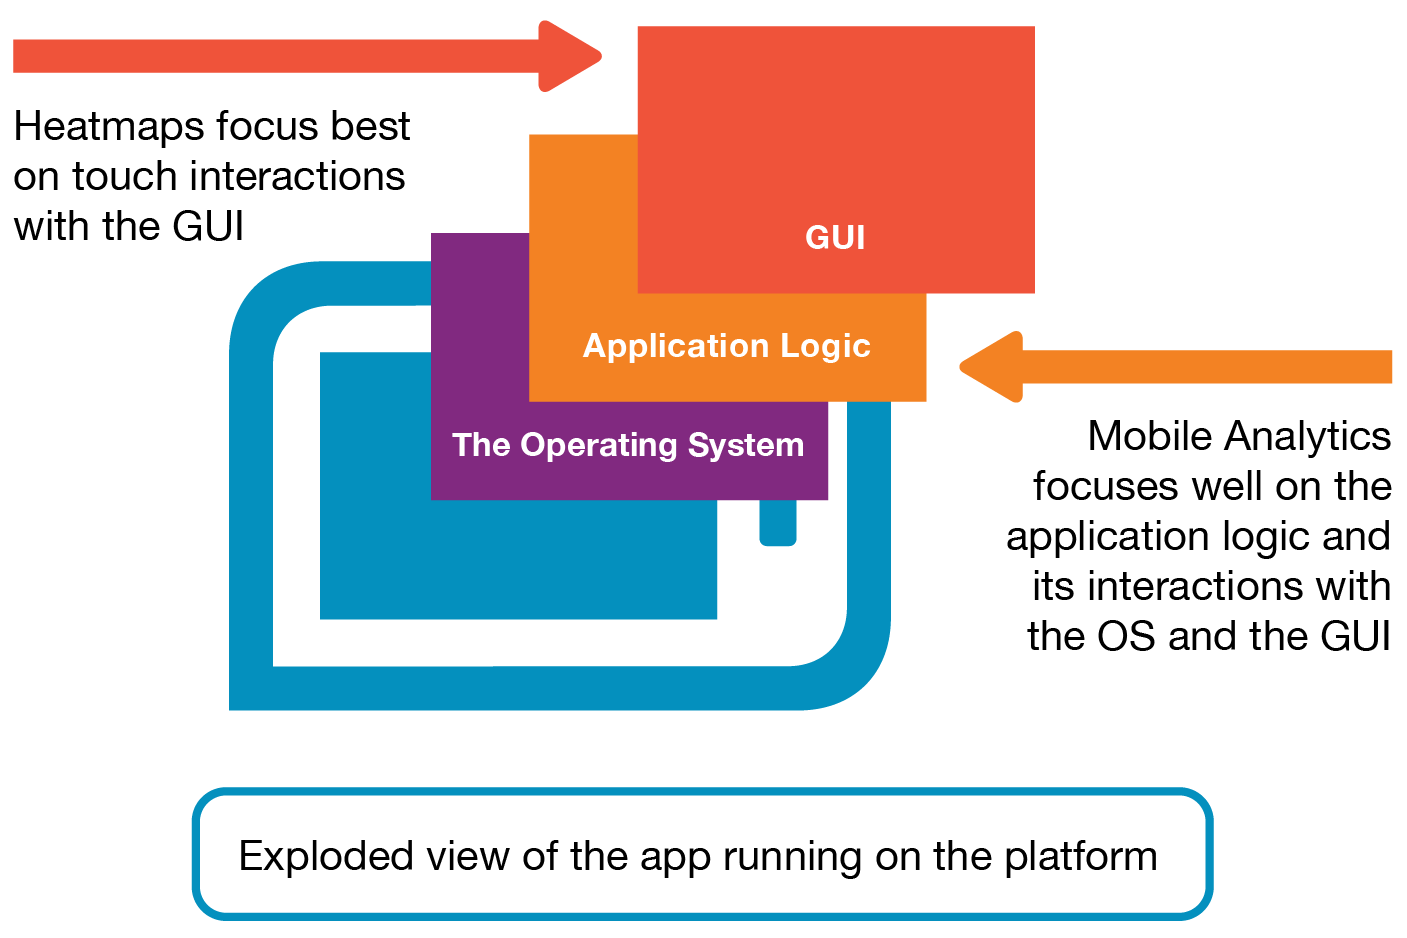
\includegraphics[width=10cm]{images/3-layers.png}
    \caption{Three layers of an app~\cite{harty_aymer_playbook_2016}}
    \label{fig:3-layers}
\end{figure}

Figure \ref{fig:3-layers} illustrates three primary observation points, or layers, for a mobile app. 

The Graphical User Interface (GUI) % SHOULD-DO add to glossary.
can be visually observed by sighted users, it can also be observed by Accessibility software, and test automation tools, \emph{etc.} externally to the app. It can also be observed from within the app, for instance through using software known as \emph{heatmapping} that records the screens and the touch interactions performed by users of that screen. One of the the more popular, mature heatmapping offerings is from AppSee~\footnote{\url{  https://www.appbrain.com/stats/libraries/details/appsee/appsee}}, nonetheless they are only used in a small minority of mobile apps.

The application may incorporate logging and/or mobile analytics. Logging in mobile apps is often used locally, by developers independently of other mechanisms. 
\begin{itemize}
    \item Logging: enables developers to understand what their software is doing. The practice is commonplace across many software domains including mobile apps, and each platform and language includes a standard method of generating log messages. These messages tend to be small and intended for immediate, local consumption. On Android when developers use the standard logging library (\texttt{android.util.log}) their log messages are written to a shared circular log file on a device. Some privileged Android software is able to read these shared logs, developers can also read them using standard Android development tools \emph{e.g.} \texttt{adb logcat} providing they are connected to the device with the log file. Older versions of Android allowed apps to read the full contents, more recently apps are restricted to only the log messages they wrote unless they are granted the relevant permission by Google and the user. 
    In other domains \emph{e.g.} web servers, infrastructure software, and many others, logging is used for production monitoring, fault-finding and analysis. A minority of mobile app developers use remote logging.
    \item Mobile analytics, can extend and scale logging. For mobile analytics, a minority of developers incorporate custom implementations, however the vast majority who use analytics do so through using third-party analytics libraries such as Google Firebase Analytics, details of the current usage of analytics libraries are provided by AppBrain~\footnote{\url{https://www.appbrain.com/stats/libraries/tag/analytics/android-analytics-libraries}}.
\end{itemize}

Similar to the concept of black box testing (where software's behaviour is observed and assessed without knowing the internals), external software can observe the behaviours of apps. Google have developed and integrated software that monitors apps running in Google approved versions of Android. The data is collected per device and provided automatically to Google servers if the device has the relevant settings enabled~\cite{google_play_share_usage_and_diagnostics_info_with_google}. This data is processed by Google who provide some portions of the data to the registered developers of that app in the Google Play Store.

\emph{Idea for expansion:} Drop-off in data for a population  c.f. marketing funnels, funnels for shopping carts, etc.

\section{Overview of applying analytics to development practices}
\begin{itemize}
    \item Decide whether to incorporate analytics into the app, and if so what data to collect, which analytics library/libraries to incorporate and the many associated aspects we will cover in this chapter.
    \item Consider whether and how to test analytics and whether to filter [out] analytics during automated and internal testing.
    \item Use and analyse the analytics data from the app and the platform (where available).
    \item Triage and prioritise potential issues reported from external sources (pre-launch testing, new releases, active mainstream releases, etc.)
\end{itemize}

\section{An aside on packaging mobile apps}
Mobile apps are a bit like snails, who carry everything with them in their shell, well actually in their application binary package (known as an APK~\footnote{Android Package Kit\url{https://en.wikipedia.org/wiki/Android_application_package}} file). This includes whichever libraries they use. Therefore, when developers want to include pre-packaged support for crash-reporting and/or mobile analytics, the development team need to incorporate the relevant software libraries in their application binary package. These libraries are therefore distributed as an intrinsic part of an app and installed seamlessly with the main application onto a user's device.

\section{Applying a crash-reporting library}
As mentioned in the section on packaging mobile apps, crash-reporting libraries need to be incorporated into an application before they can be used. Generally~\footnote{A small minority of developers may follow other practices, nonetheless the principles mentioned here still apply}, the developer adds a few configuration lines to their application's build file (in \texttt{app/build.gradle} for Android apps) and also several lines of code to initialise the library when the application starts. These install the library as the global crash handler for the app, each time the app is started the library is initialised. 

When the library is initialised, it may perform various actions such recording details of the operating system release, the model of device, \emph{etc.}. They may also perform house-keeping activities, for instance Crashlytics transmits crash reports from previous sessions.

Some crash-reporting libraries offer developers an API to add \emph{breadcrumbs} at run-time. If/when a crash occurs and is reported, the immediately preceding breadcrumb data may help developers piece together possible causes for a particular crash.

Some crash-reporting libraries offer developers a mechanism to report non-fatal crashes: caught exceptions. These would be handled by the application yet be considered noteworthy and worthy of analysis by the development team. A good example of a library that includes support for non-fatal crash reporting is the popular Crashlytics offering.  

\subsection{Testing crash-reporting}
\begin{itemize}
    \item Sanity test
    \item Latency
\end{itemize}

Testing a system intended to measure quality may adversely affect their rating of your apps and potentially even their willingness to accept you in their system. \emph{c.f.} credit checks may adversely affect your credit score score~\footnote{\url{https://www.experian.co.uk/consumer/guides/searches-and-credit-checks.html}}. The system may not distinguish between your testing of the measurement system and those experienced by end users of the software. Google is adamant they will not accept Android apps that crash: ~\emph{``\textbf{Broken Functionality} We don’t allow apps that crash, force close, freeze, or otherwise function abnormally."}~\cite{google_play_developer_policy_center}.

\section{Designing logging}
\subsection{Testing logging}

\section{Designing in-app analytics}
\subsection{Testing in-app analytics}

\section{An aside on 'pre-launch reports'}
Google provide a free service called pre-launch reports~\cite{google_use_pre_launch_reports}. TBC.
\section{Selecting Mobile Analytics}

\begin{itemize}
    \item Establish the selection criteria \emph{e.g.} the intended goals and purposes of the data collection, compare with non-functional qualities, flexibility of the API, price, privacy, licensing, legal, and other selection criteria.
    \item Establish the acceptance criteria, including any design and implementation aspects.
    \item TBC...
\end{itemize}

\section{Summary of applying analytics to development practices}



\section{Evaluation of the case studies framed through the contents of this chapter}
